\documentclass[9pt,journal,a4]{IEEEtran}

\usepackage{cite}
\usepackage{amsmath}
\usepackage{graphicx}
\usepackage{textcomp}
\usepackage{color}
\usepackage{soul}
\usepackage{booktabs}
\graphicspath{{figures/}}

\begin{document}

\title{From Individual Uncertainty to Collective Predictability: The Impact of Temporal and Population Aggregation on Temperature-Driven Thermostatic Loads}


\author{Alexandre~M.~V.~Gouveia}

\maketitle

\begin{abstract}
% TODO
\end{abstract}

\begin{IEEEkeywords}
Electric thermostatic loads, heat pumps, low-voltage networks, degree-day regression, smart meter data, distribution system observability.
\end{IEEEkeywords}


\section{Introduction}

\begin{itemize}

\item \textbf{Macro driver.}

Electrification of heating and cooling, driven by decarbonisation policy.


\item \textbf{Concession then problem.}

Electric Thermostatic Load (ETL) uptake is a positive driver for decarbonisation, yet introduces temperature-correlated demand on low-voltage (LV) networks not sized for it.


\item \textbf{Narrow to the gap.}

Distribution System Operators (DSOs) hold net-load and weather data at the substation, and the thermal response of an ETL population is in principle visible in it. What is generally absent is the context needed to interpret that response: appliance registers, nameplate ratings and, critically, the number of consumers the substation serves. Concrete figures on registry coverage should be provided here.

The aggregation level is consequently not a fixed property of the problem but an unknown that varies between substations, and it governs both how clearly the thermal response appears and how ambiguous its origin is.


\item \textbf{Literature in named categories.}

The relevant literature should be organised into the following categories:

\begin{itemize}

\item Load Disaggregation;

\item Change-Point and Degree-Day Regression; and

\item Diversity and Simultaneity in Network Planning.

\end{itemize}

A non-exhaustive summary table of prior work should also be included.


\item \textbf{Gap, contributions, and roadmap.}

Previous work establishes the load--temperature relationship using submetered thermal load, where the thermal contribution is directly observable, or at a single fixed level of aggregation. The aggregation level itself has not been treated as the variable that governs what remains identifiable.

This paper makes three contributions:

\begin{enumerate}

\item It formalises consumer aggregation as the governing variable in the identifiability of Electric Thermostatic Loads from aggregated LV net load, separating the predictability that aggregation confers from the attributability it removes.

\item It implements two use cases derived from a single fit, namely Detection and Energy Estimation, and reports each as a function of the aggregation level. Each is scored against submetered ground truth, yet requires only net load and ambient temperature to be applied.

\item It reproduces the aggregation effect on two further previously unseen datasets, drawn from different climates and building stocks, one of them driven by cooling rather than heating, using nested sequences of aggregates and without recalibrating the fitting procedure.

\end{enumerate}

\item \textbf{Roadmap.}

The rest of the paper is structured as follows: Section~\ref{section:identify} formalises the thermal response of aggregated net load and the two opposing effects of consumer aggregation; Section~\ref{section:aggregation} describes the data and measures how aggregation improves the fit, reproducing the effect on two unseen datasets; Section~\ref{section:usecases} reports the two use cases against aggregation level; in Section~\ref{section:discussion}, accuracy, generalisability, data requirements and interpretability are discussed. Lastly, Section~\ref{section:conclusion} concludes the paper.

\end{itemize}

\section{Aggregation and the Identifiability of Thermal Loads}
\label{section:identify}

In this section, the thermal response of aggregated LV net load is formalised. Consumer aggregation is then shown to act on this response in two opposing directions, and the two use cases implemented in the remainder of this paper are derived from the tension between them.


\subsection{Thermal Response of Aggregated Net Load}

ETLs, a class comprising heat pumps, direct resistive heating and electric cooling, modulate their electrical consumption in response to ambient temperature. At the individual consumer level this behaviour is thermostatically controlled and strongly intermittent: a single ETL is either running or idle, and its instantaneous demand is a poor indicator of the temperature that caused it. Aggregation over the consumers downstream of an LV substation removes that intermittency. Thermostatic cycling decorrelates between dwellings and idiosyncratic occupancy averages out, so the aggregate response becomes smooth and approximately piecewise linear in temperature.

The model below is therefore a description of a population rather than of a consumer, and the size of that population is a condition for the model to hold at all rather than an incidental detail.

Aggregated net load is modelled as
\begin{equation}
P(T)
=
P_{\mathrm{base}}
+
s_h \max\left(0,T_h-T\right)
+
s_c \max\left(0,T-T_c\right),
\label{eq:thermal-response}
\end{equation}
where $P$ is the aggregated net load [kW], $T$ is the ambient temperature [$^\circ$C], $P_{\mathrm{base}}$ is the temperature-independent component [kW], $s_h$ and $s_c$ are the heating and cooling Thermal Sensitivities [kW/$^\circ$C], and $T_h$ and $T_c$ are the corresponding threshold temperatures [$^\circ$C]. The interval $[T_h,T_c]$ is a dead band over which no thermal response is present, with $T_h \leq T_c$ imposed during fitting. The $\max\left(0,T_h-T\right)$ and $\max\left(0,T-T_c\right)$ terms are also called Heating Degrees (HD) and Cooling Degrees (CD), respectively.

Equation~\eqref{eq:thermal-response} describes a V-Shaped Fit. Where no electric cooling is installed, $s_c$ is zero, and the expression reduces to a Hockey-Stick Fit observed in low temperatures. Similarly, when no electric heating is present, $s_h$ is zero, and only the cooling portion of the fit is observed.

Fig.~\ref{fig:bathtub} shows the full V-Shaped form recovered from measured data, on an aggregate of 22 air-conditioned dwellings in Austin, Texas. Both arms and the intervening dead band are present: a heating sensitivity of 0.68~kW/$^\circ$C below $T_h = 11.2^\circ$C, a cooling sensitivity of 3.05~kW/$^\circ$C above $T_c = 19.8^\circ$C, and a flat interval between the two.

The two arms are not produced by the same device, and only one of them is an ETL. Circuit-level submetering attributes the cooling arm to the air conditioners, whereas 21 of the 22 dwellings draw essentially nothing on that circuit in winter. The heating arm comes instead from the furnace circuits, which the dataset defines as furnace and air handler combined, at a median 0.08~kW per dwelling in cold weather. No dwelling in the pool carries a dedicated electric heater circuit and gas service is recorded for most, so that draw is an air handler rather than electric resistance heat, and the heat itself never reaches the electricity meter. Equation~\eqref{eq:thermal-response} describes the aggregate response in either case, which is what the figure is shown for, though the distinction matters wherever an arm is read as evidence of an ETL.

\begin{figure}[t]
\centering
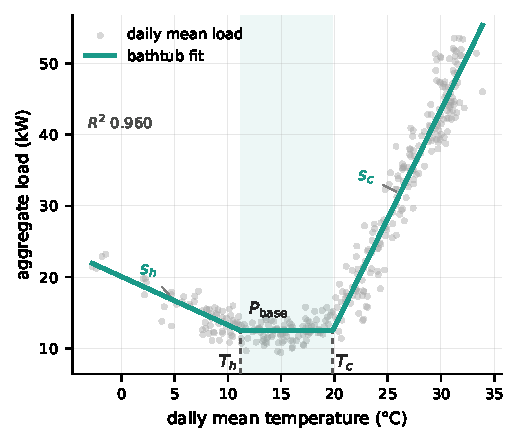
\includegraphics[width=\columnwidth]{figures/fig_bathtub_example.pdf}
\caption{Equation~\eqref{eq:thermal-response} fitted to an aggregate of 22 air-conditioned dwellings in Austin, Texas, over calendar year 2018. Both arms and the dead band (shaded) are identified from the data.}
\label{fig:bathtub}
\end{figure}

\subsection{The Two Effects of Consumer Aggregation}
\label{subsection:two-effects}

The first effect of increasing the consumer count $N$ is to improve how well Equation~\eqref{eq:thermal-response} describes the data. Averaging over more consumers suppresses the idiosyncratic component of demand while leaving the temperature-driven component intact, since only the latter is common to every consumer downstream of the substation. The fitted parameters are correspondingly better determined. Section~\ref{section:aggregation} quantifies the improvement in the fit and in the spread of the parameters alike, and in each the gain is largest where ETL penetration is lowest.

The second effect runs the other way. The aggregated sensitivity is the sum of the individual sensitivities of all consumers downstream of the substation, and consumers without an ETL are not thermally inert. Lighting and occupancy patterns correlate with the seasonal temperature cycle, so a small positive sensitivity remains even in the absence of ETLs. The heating sensitivity is therefore decomposed as
\begin{equation}
s_h
=
N \sigma_{\mathrm{base}}
+
N_{\mathrm{etl}} \sigma_{\mathrm{etl}},
\label{eq:sensitivity-decomposition}
\end{equation}
where $N$ is the number of consumers downstream of the substation, $N_{\mathrm{etl}}$ is the number of those consumers with an ETL, $\sigma_{\mathrm{base}}$ is the mean per-consumer non-thermal sensitivity, and $\sigma_{\mathrm{etl}}$ is the mean per-load thermal sensitivity.

The residual per-consumer term is more than an order of magnitude smaller than the per-load term, yet it accumulates with substation size. A large substation with no ETLs may consequently exhibit a sensitivity comparable to a small substation with high ETL penetration. A given value of $s_h$ is thus consistent with many $(N, N_{\mathrm{etl}})$ pairs, and neither quantity is generally known to the DSO. Aggregation therefore buys a better-determined curve at the cost of a more ambiguous one.

These two effects do not carry equal weight. What Equation~\eqref{eq:sensitivity-decomposition} obstructs is not identification at a large $N$, but identification at an unknown $N$: were the consumer count published alongside the aggregated consumption, the reference contribution $N \sigma_{\mathrm{base}}$ could be subtracted and the ambiguity would not arise. Section~\ref{subsection:detection} separates the two, by comparing substations of equal and known size against the same substations pooled over an unknown one.

The obstruction is consequently addressable without recovering $N$ itself. Normalising $s_h$ by an observable that scales with $N$, such as the substation peak load or the fitted base load $P_{\mathrm{base}}$, removes most of the dependence. This route is adopted here, since it remains applicable where no consumer count is published alongside the aggregated consumption.

Aggregation over time acts on the same trade-off, and for the same reason. Fitting is performed on daily aggregates rather than at the native measurement resolution, since averaging over a full diurnal cycle removes occupancy-driven variability that is not temperature-dependent. It also removes the effect of buildings' thermal inertia, which causes a mismatch between consumption and outdoor temperature at high resolutions. This averaging comes at the cost of intra-day detail. Consumer count and averaging window are two axes of one operation, and Section~\ref{section:aggregation} reports the fit against both.


\subsection{Identifiable Quantities and Use Cases}

The parameters of Equation~\eqref{eq:thermal-response} support two use cases. They differ in how much of the aggregation level each needs to be known, which follows directly from Equation~\eqref{eq:sensitivity-decomposition}.

\textbf{Detection.} The presence of ETLs downstream of a substation is assessed by comparing a normalised sensitivity against a reference distribution obtained from substations known to contain none.

Detection is scoped to presence alone, and the penetration rate is not inferred from the fit. Below a minimum detectable penetration, the ETL term of Equation~\eqref{eq:sensitivity-decomposition} is smaller than the spread of the reference group, and the two populations are not separable. Where that minimum lies is a property of the reference group rather than of any one substation. The design below bounds it from above rather than resolving it, since the grid does not extend to penetrations low enough for detection to fail.

\textbf{Energy Estimation.} Integrating Equation~\eqref{eq:thermal-response} over the temperature profile of a given day yields the temperature-driven energy consumed on that day. For the heating arm, this reduces to the product of $s_h$, the HD value of that day, and the number of hours over which it applies. The cooling arm follows from the equivalent product using CD. Both terms of Equation~\eqref{eq:sensitivity-decomposition} contribute to the result, so the estimate refers to the total temperature-driven energy. Isolating the ETL share requires subtracting the reference contribution $N \sigma_{\mathrm{base}}$. The dead band also bounds where the estimate can be accurate at all: above $T_h$ the thermal term is identically zero, so any ETL energy that persists into mild weather is unexplained by construction, not by a fitting failure. Section~\ref{subsection:energy} checks accuracy against both ETL penetration and the observed temperature range accordingly.

Both use cases are consequently reported against the aggregation level in Section~\ref{section:usecases}, rather than at a single one.

It should be noted that neither use case yields the installed capacity of the ETLs. Recovering capacity from a Thermal Sensitivity requires the ratio between aggregated demand and the sum of the individual rated powers, which net load alone does not identify. Capacity estimation consequently falls outside the scope of this paper.


\section{Aggregation and Predictability}
\label{section:aggregation}
In this section, the first of the two effects described in Section~\ref{subsection:two-effects} is measured. The datasets and substation designs are described first. Fit quality is then reported against consumer count on the training data, and reproduced on two further datasets drawn from different climates and building stocks.


\subsection{Datasets}
\label{subsection:data}

The training data is the HEAPO dataset, complemented with additional smart-meter data providing submetered thermal load. Both are Swiss, and together give net load at 15-minute resolution for 1702 LV consumers over calendar year 2023. Of these, 395 have an ETL, of which 81 carry a submetered heat pump. Heat pumps are the only ETL used in this paper, since they are the only ETL technology with a submetered thermal series in either dataset: the heat pump is the only device paired to a household meter in this data. The remaining 314 ETL-equipped consumers are identified from survey flags alone and are not used in the substation designs below. Ambient temperature is available hourly, which sets 1~h as the finest resolution at which the fit is evaluated.

A consumer is classified as ETL-free where it carries no submetered heat pump and none of five labelled electric heating types is recorded in the household survey: electric water heater, storage heating, direct heating, auxiliary heat pump and water-heating heat pump. This leaves 1307 ETL-free consumers. The negative class is therefore defined rather than filtered, which a heat-pump-specific framing would not achieve, since a consumer with resistive heating would remain in the reference group and contaminate it.

The validation data is WPUQ, 37 German single-family houses on one low-voltage feeder, each with separately metered heat pump and household circuits, over calendar year 2019. Ambient temperature is recorded at five-minute resolution against the training data's hourly series, though every fit in this paper rests on hourly temperature at the coarsest, so the difference does not propagate into the results. The data predates the German regulatory provisions for controllable heat pump loads that came into force in 2024.

A third dataset supplies the cooling arm, which neither of the others contains. Pecan Street's Austin panel gives 22 air-conditioned dwellings in Texas over calendar year 2018 at 15-minute resolution, each with circuit-level submetering. Its air conditioners are a genuine ETL and dominate the summer load, drawing 25~kW summed over the pool above 25$^\circ$C against 1~kW below 10$^\circ$C. Its heating arm is not an ETL, for the reason given in Section~\ref{section:identify}, so Austin is used to test the aggregation claim on a cooling-driven fit rather than to add a second heating population.

Neither Swiss nor WPUQ consumers carry a labelled cooling load, and the summer behaviour of the WPUQ heat pumps is consistent with this. Pooling its 37 units over June-August, the correlation between load and temperature is negative in 18 of 37 cases at $p<0.05$ against positive in 2, and the median correlation across all units is $-0.18$. The cooling sensitivity $s_c$ is consequently zero for both, and only the heating arm of Equation~\eqref{eq:thermal-response} is fitted on either. Austin is the one dataset where both arms are free.


\subsection{Substation Designs}
\label{subsection:designs}

Synthetic substations are drawn from the Swiss pool, each consumer appearing at most once within a given substation but reused freely across substations. Consumer count $N$ and ETL count $N_{\mathrm{etl}}$ are varied independently over a factorial grid of 12 sizes and 5 penetration levels, at 25 replicates per cell, giving 1500 substations. The five penetration levels are 0, 25, 50, 75 and 100\%, and the 0\% cells supply the ETL-free reference distribution against which Detection is scored in Section~\ref{subsection:detection}. Every substation is tied to a single weather station, so that one temperature series applies to all of its members. The 81 submetered heat pumps are split across stations and the largest holds 50 of them, which caps $N$ at 48 for the fully penetrated cells, where $N_{\mathrm{etl}} = N$.

The design does not exhaust the pool. Drawing is confined to one weather station per substation and stops at $N = 48$, so 1384 of the 1702 consumers and 77 of the 81 submetered heat pumps are actually used, and every figure below refers to those.

The 1500 substations are also not 1500 independent observations. They are built from those 1384 consumers, of which only the 77 carrying a submetered heat pump ever supply the ETL tier, so each of the 77 appears in approximately 250 substations. Reuse is also uneven across the grid rather than uniform. Replicates within a cell share a mean 3\% of their ETL members at $N = 4$ and 25\% penetration, against 92\% at $N = 48$ and full penetration. At that corner 48 members must be drawn from the 50 heat pumps the station holds. The design is consequently a controlled traverse of the $N \times N_{\mathrm{etl}}$ grid rather than a sample of a substation population, and the replicates suppress the variability of the draw rather than measure that of the consumer population. The Detection interval reported in Section~\ref{subsection:detection} is therefore obtained by resampling consumers rather than substations. Comparisons that hold the consumers fixed and vary something else, such as the resolution comparison of Section~\ref{subsection:resolution}, are paired and do not inherit the same difficulty.

WPUQ cannot support the same design, and what it can support is set by what it contains. Every household carries a heat pump, so a reference group of genuinely ETL-free consumers cannot be assembled: withholding a household's own heat pump circuit would yield a negative class that differs from the positive one by that circuit alone, with the entire non-thermal load held identical. Detection scored against such a class would be an easier problem than the one Section~\ref{subsection:detection} poses, and would report an optimistic figure for that reason rather than because the threshold transfers. Detection is consequently evaluated on the training data alone.

The aggregation claim carries no such difficulty, since it concerns how the fit responds to consumer count rather than how two classes separate. It is tested on WPUQ with one substation per aggregation level, in a nested sequence: the aggregate at $N$ contains the aggregate at $N-4$, so each step is the addition of four consumers to a fixed set rather than a comparison between independent draws. Roles are fixed before any aggregate is built, half the pool contributing its heat pump circuit and half having it withheld, which holds penetration at 50\% throughout and matches the condition reported for the training data below.

Nine substations result, from $N = 4$ to $N = 36$. No replicates are drawn and none are implied. A factorial design over the same 37 houses would yield a larger substation count without a corresponding gain in evidence, for the reason just given. The single nested sequence instead makes the dependence on $N$ visible without inviting a precision claim the pool cannot support.

Austin is aggregated the same way, in a nested sequence from $N = 4$ to $N = 22$ in steps of two. There is no penetration to hold fixed, since every dwelling in the pool has an air conditioner, so each level is simply the first $N$ of one fixed random ordering. Both arms of Equation~\eqref{eq:thermal-response} are fitted at every level.

Every result on the training data is evaluated on the same calendar year the parameters were fitted on, with no held-out period. This is not a like-for-like restatement of the fit, since the fit target is net load throughout, whereas Detection is scored against a labelled reference group and Energy Estimation against submetered thermal energy the fit never sees. It does mean those figures carry no penalty for temporal extrapolation. WPUQ supplies the genuinely out-of-sample test, on a dataset from a different year, country and building stock.

Network losses between the consumers and the substation are neglected. However, since the objective is to obtain realistic substations rather than exact recreations of a particular network, this assumption is reasonable. The WPUQ feeder carries a measured transformer against which the synthetic aggregation can be checked directly: its 37 monitored households account for 49.5\% of the transformer's mean load and the two series correlate at 0.95, so the monitored set behaves as a substantial and representative fraction of a real feeder.


\subsection{Fit Quality Against Aggregation Level}
\label{subsection:fitquality}

The effect is directly observable on the training data. Median net-load $R^2$ at 24~h rises with the consumer count at every penetration level: from 0.710 at $N = 4$ to 0.921 at $N = 48$ for substations at 25\% penetration, and from 0.856 to 0.948 at 50\%. The gain is largest where the ETL signal is weakest. At full penetration the same range yields only 0.925 to 0.958, since the response is already well determined by the ETLs alone.

The reference group shows the effect in isolation. Substations carrying no ETL reach a median $R^2$ of 0.188 at $N = 4$ against 0.524 at $N = 48$, so aggregation renders identifiable a temperature response that no ETL produces. This is the $N \sigma_{\mathrm{base}}$ term of Equation~\eqref{eq:sensitivity-decomposition} becoming a well-determined curve in its own right, and it is why the quality of a fit is not by itself evidence of ETL presence.

The fitted parameters stabilise alongside the fit. The relative interquartile spread of $s_h$ across the replicates of a cell falls from 0.365 to 0.223 between $N = 4$ and $N = 48$ at 25\% penetration, and from 0.368 to 0.122 at 50\%. The corresponding figures at higher penetration are not reported here, since replicates there are drawn from a nearly exhausted pool and agree with one another for the reason given in Section~\ref{subsection:designs}, rather than because the estimate has converged.

Fig.~\ref{fig:aggregation-quality} places the consumer axis alongside the temporal one, at a fixed 50\% penetration. Both act in the same direction, which is what justifies treating consumer count and averaging window as two forms of one operation rather than as unrelated design choices. They are also partly interchangeable. Raising the consumer count from 4 to 48 gains 0.410 in $R^2$ at 1~h resolution, against 0.092 at 24~h, so much of what aggregating consumers achieves has already been achieved by averaging over time. Over part of their range the two are consequently substitutes rather than independent improvements, an interaction Section~\ref{subsection:reproduction} finds holds in one further dataset but not the other. Section~\ref{subsection:resolution} returns to the cost attached to the temporal axis.

\begin{figure}[t]
\centering
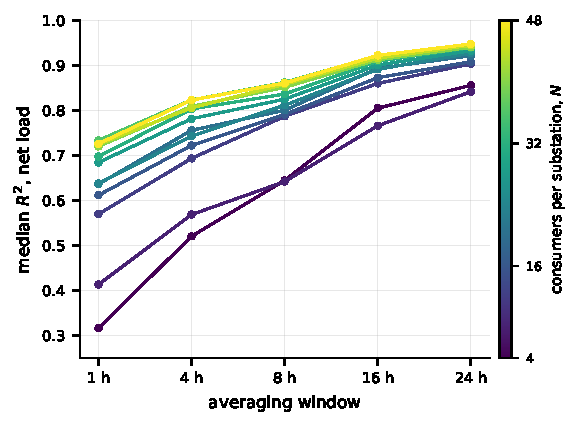
\includegraphics[width=\columnwidth]{figures/fig_aggregation_quality.pdf}
\caption{Median net-load $R^2$ against averaging window, one line per consumer count, at a fixed 50\% ETL penetration. Both aggregation axes act in the same direction, and they partly substitute for one another: the spread between consumer counts narrows as the averaging window widens.}
\label{fig:aggregation-quality}
\end{figure}


\subsection{Reproduction on Independent Datasets}
\label{subsection:reproduction}

Fit quality rises with the consumer count at every averaging window in WPUQ as well (Fig.~\ref{fig:nested-aggregation}, left). At 24~h, net-load $R^2$ goes from 0.667 at $N = 4$ to 0.845 at $N = 36$, and at 1~h from 0.499 to 0.605. The direction is the same on a dataset the fitting procedure has never seen, with no recalibration of bounds and no adjustment to the fit.

\begin{figure*}[t]
\centering
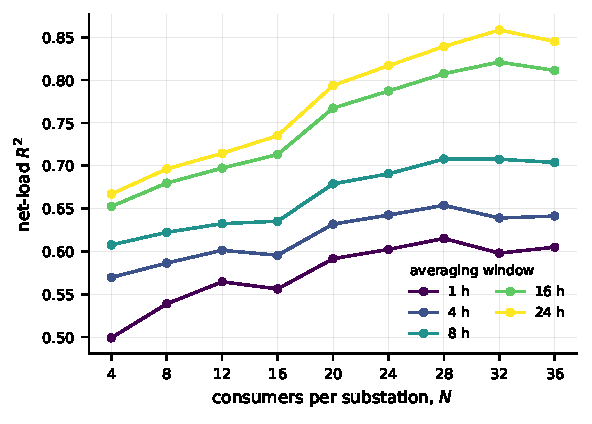
\includegraphics[width=\textwidth]{figures/fig_nested_aggregation.pdf}
\caption{Net-load $R^2$ against averaging window for the two nested sequences, one line per consumer count, drawn on the axes of Fig.~\ref{fig:aggregation-quality}. Left: WPUQ, heating arm only, at 50\% ETL penetration. Right: Austin, both arms of Equation~\eqref{eq:thermal-response} free. Each aggregate contains the one below it, so a lighter line is a strict superset of a darker one. No band is shown because there are no replicates.}
\label{fig:nested-aggregation}
\end{figure*}

Austin reproduces the same direction with both arms free (Fig.~\ref{fig:nested-aggregation}, right). Net-load $R^2$ at 24~h rises from 0.799 at $N = 4$ to 0.958 at $N = 22$, increasing at every step but a negligible dip at $N = 18$. The gain is steepest below $N = 10$ and the curve is nearly flat beyond, so most of what aggregation offers is obtained within the first dozen consumers. Reading across consumer counts rather than along the window, the rise is not strictly monotone in either dataset, which is expected of single realisations: an individual consumer added at one step may be less regular than the aggregate it joins, an irregularity the training data averages away over its replicates.

The figures also make the two-axis interaction visible, as the degree to which the lines converge from left to right. In the training data the consumer-count effect shrinks as the window widens, from 0.410 in $R^2$ at 1~h to 0.092 at 24~h, so the lines fan in and the two axes act as substitutes. Austin behaves the same way, the consumer-count effect falling from 0.261 to 0.159 over the same range. WPUQ is the exception: there the effect grows, from 0.106 to 0.178, and the lines fan out rather than in. The substitution therefore holds in two datasets of three. Its failure in WPUQ might indicate that those fits remain limited at fine resolution by something other than consumer count, its individually metered single-family houses having sharper sub-daily swings than a mixed consumer pool.

The two arms of the Austin fit do not sharpen at the same rate, which is instructive. The cooling threshold $T_c$, belonging to the air conditioners, settles at 19.8$^\circ$C and varies by a standard deviation of 0.10$^\circ$C once $N \geq 10$. The heating threshold $T_h$, belonging to no thermostatic load at all, wanders between 10.1 and 11.3$^\circ$C over the same range, at a standard deviation of 0.51$^\circ$C. Aggregation sharpens the parameter describing a real thermostatic population and leaves the other loose, which is the same asymmetry the reference group of Section~\ref{subsection:fitquality} shows from the opposite direction.

Aggregation therefore confers predictability regardless of dataset, climate, building stock or thermostatic technology.

\subsection{Coincidence of the Heat Pump Population}
\label{subsection:simultaneity}

A third quantity follows the same transition, and it is the one aggregation is classically expected to govern. The Simultaneity Factor (SF) is the fraction of a population's connected load drawing power at once, fitted here in the same three-parameter form as the net-load response, against submetered heat pump load normalised by its installed peak. At the individual level the quantity is degenerate, since a single heat pump is either running or idle and its coincident fraction is therefore 0 or 1. Aggregation is what renders it a stable fraction of the connected load.

Fig.~\ref{fig:simultaneity} reports the fitted SF at each substation's coldest observed day, against the number of heat pumps aggregated. The median is almost flat, moving from 0.38 at a single heat pump to 0.42 by a dozen and holding there. The spread is what changes, with the interquartile range across substations narrowing from 0.162 at one heat pump to 0.007 at 48. Aggregation does not so much reveal a coincidence value as render a fixed one certain, which is the SF reading of the individual-to-collective transition the rest of this section describes.

\begin{figure}[t]
\centering
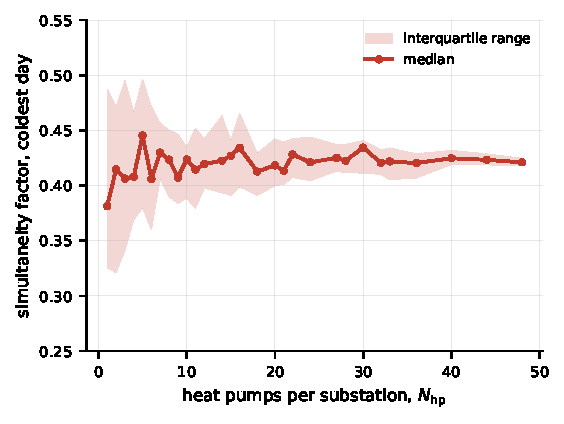
\includegraphics[width=\columnwidth]{figures/fig_sf_by_aggregation.pdf}
\caption{Fitted simultaneity factor at each substation's coldest observed day, against the number of heat pumps aggregated, on the training data. The median holds near 0.42 while the interquartile band funnels in, from 0.162 at a single heat pump to 0.007 at 48.}
\label{fig:simultaneity}
\end{figure}

The collapse is not an artefact of the replicate reuse noted in Section~\ref{subsection:designs}. Restricting to 25\% penetration, where replicates share at most 14\% of their heat pumps, the interquartile range still falls from 0.162 at one heat pump to 0.038 at twelve. The reuse only reinforces the further tightening seen at the largest counts.

The SF is reported here to characterise the aggregation rather than as an operating quantity, since it is built from the submetered heat pump load and its installed peak, neither of which a DSO holds. Its absolute level reflects the local climate and heat pump sizing rather than a value that transfers across networks, in the same way as the absolute Thermal Sensitivities discussed in Section~\ref{subsection:generalisability}. Converting it into an available flexibility would additionally require the installed capacity it is a fraction of, which Section~\ref{section:identify} notes net load does not identify. What aggregation delivers is the predictability of the coincidence, not its magnitude in kilowatts.

Across these readings -- fit quality, parameter spread and coincidence alike -- aggregation supplies predictability rather than a value to be recovered. The following section turns to what that predictability is worth: the quantities the resulting fit makes identifiable, and the aggregation level at which each becomes usable.


\section{What Aggregation Makes Identifiable}
\label{section:usecases}
In this section, the two use cases introduced in Section~\ref{section:identify} are implemented. Both read the fit whose behaviour Section~\ref{section:aggregation} established, so each is reported against the aggregation level rather than at a single one. Both are evaluated on the training data, for the reason given in Section~\ref{subsection:designs}.


\subsection{Detection}
\label{subsection:detection}

The median sensitivity surface over the $N \times N_{\mathrm{etl}}$ grid is shown in Fig.~\ref{fig:confound}. A least-squares fit of Equation~\eqref{eq:sensitivity-decomposition} across this surface, constrained through the origin as the equation requires, gives $\sigma_{\mathrm{base}} = 0.0054$~kW/$^\circ$C per consumer and $\sigma_{\mathrm{etl}} = 0.117$~kW/$^\circ$C per ETL, at $R^2 = 0.999$. A single ETL is therefore worth approximately 22 ordinary consumers of raw sensitivity. The size dependence is severe enough to invert a ranking: a 48-consumer substation with no ETL reaches 0.27~kW/$^\circ$C, exceeding the 0.24~kW/$^\circ$C of a 4-consumer substation at 50\% penetration. Raw sensitivity is consequently not interpretable as evidence of ETL presence without independent knowledge of $N$, which motivates the normalisation adopted below.

\begin{figure*}[t]
\centering

\includegraphics[width=\textwidth]{figures/fig3_confound.pdf}
\caption{Median net-load thermal sensitivity over the $N \times N_{\mathrm{etl}}$ grid, on a logarithmic colour scale. Rows are ETL penetration and columns the consumer count $N$.}
\label{fig:confound}
\end{figure*}

Median raw sensitivity is 0.122~kW/$^\circ$C for substations containing no ETL, against 1.681~kW/$^\circ$C for those containing at least one, and the two distributions overlap across the whole lower range. Normalising by peak load separates them with an Area Under the Curve (AUC) of 0.990, against 0.974 for the raw statistic, at sensitivities of 0.958 and 0.875 respectively at 95\% specificity (Fig.~\ref{fig:detection}, left). Resampling consumers with replacement, stratified by weather station and ETL status, then redrawing the design and refitting, gives a 95\% percentile interval of $[0.970, 0.996]$ on the former over 200 replicates. Resampling substations instead would give $[0.983, 0.995]$, less than half as wide: the same 77 submetered heat pumps recur in every substation-level replicate, so only consumer-level resampling reaches the variability described in Section~\ref{subsection:designs}. Normalising by the fitted base load performs comparably, at an AUC of 0.987 and a sensitivity of 0.979.

These pooled figures understate what the fit recovers, since they mix substations of different and unknown size. Computing the same AUC within each consumer count separately, so that positives and negatives share a known $N$, gives a median of 1.000 for the raw sensitivity across the 12 sizes (Fig.~\ref{fig:within-stratum}). It reaches exactly unity in 8 of them and never falls below 0.990. Separation is therefore essentially perfect at every aggregation level tested, including the smallest at $N = 4$. The difficulty Detection faces is not a large $N$ but an unknown one, as Section~\ref{subsection:two-effects} anticipated.

\begin{figure}[t]
\centering
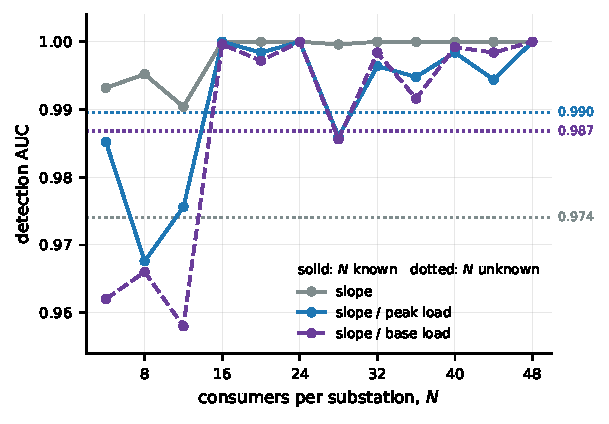
\includegraphics[width=\columnwidth]{figures/fig_within_stratum_auc.pdf}
\caption{Detection AUC against consumer count, scored within each count separately so that positives and negatives share a known $N$ (solid), against the same statistic pooled over every $N$ (dotted). The vertical distance between a pair is the cost of not knowing $N$, and the ranking of the three statistics inverts between the two views.}
\label{fig:within-stratum}
\end{figure}

The gap between the two views measures that difficulty directly. For the raw sensitivity it is 0.026, from a within-size median of 1.000 to a pooled 0.974. Peak normalisation reduces the gap to 0.006 and base normalisation to 0.011, so roughly three quarters of the loss is recoverable without knowing $N$. The ranking of the three statistics consequently inverts between the two views: the raw sensitivity is the best discriminator at known $N$ and the worst at unknown $N$, since normalising by a noisy observable costs accuracy where no size correction is needed.

This also settles the choice between the two normalisers. Base normalisation separates marginally better at known size, at a median of 0.998 against 0.996. Peak normalisation is nonetheless the more effective correction for size being unknown, which is the condition under which the statistic is deployed.

Detection against penetration is shown in Fig.~\ref{fig:detection}, right. At the same operating point, the detection rate reaches 0.87 at 25\% penetration, 0.97 at 50\% and unity above 75\%. The 25\% level is the lowest this design realises, so the minimum detectable penetration is bounded above by that figure rather than resolved by it.

\begin{figure*}[t]
\centering
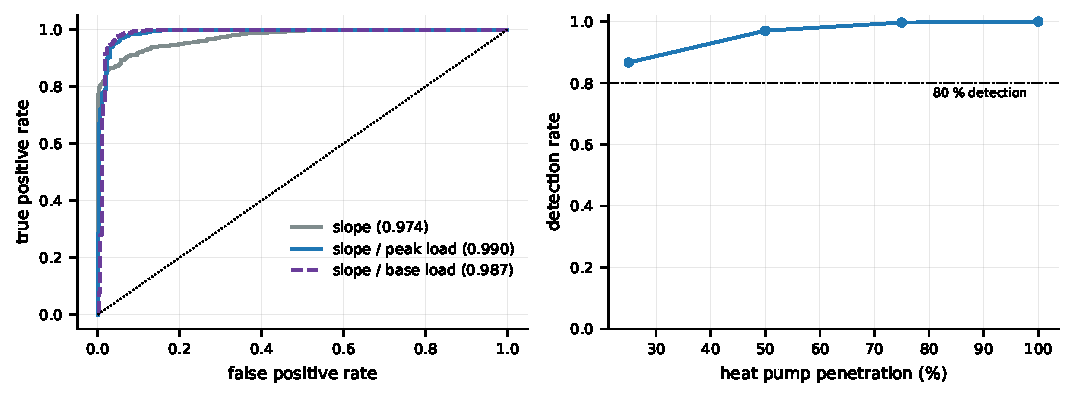
\includegraphics[width=\textwidth]{figures/fig4_detection_train.pdf}
\caption{Left: Receiver Operating Characteristic (ROC) curves for the raw thermal sensitivity and for the two normalised variants. Right: detection rate against ETL penetration at 95\% specificity.}
\label{fig:detection}
\end{figure*}

A specificity of 95\% is nevertheless a weak guarantee where ETL deployment is sparse. Holding the observed sensitivity and specificity fixed, the Positive Predictive Value (PPV) is 0.16 at a deployment prevalence of 1\%, 0.50 at 5\% and 0.68 at 10\%. Below roughly 5\% prevalence, most flagged substations are therefore false positives, and the statistic is better used to rank substations for inspection than to classify them outright.


\subsection{Energy Estimation}
\label{subsection:energy}

Pooled across 438\,000 substation-days, the thermal term of Equation~\eqref{eq:thermal-response} reaches $R^2 = 0.953$ against submetered thermal energy, at a total-energy bias of $-11.5\%$ and a Root Mean Square Error (RMSE) of 91~kWh/day. The estimate is built from the day's mean temperature alone, and is compared against a quantity the fit never saw, since the fit target was net load rather than thermal energy.

Table~\ref{tab:energy-penetration} reports the estimator against ETL penetration, with the detection rate repeated for comparison. $R^2$ remains above 0.88 at every penetration level, whereas the detection rate falls to 0.87 over the same range. Energy Estimation is accordingly the more robust of the two use cases at low penetration, as anticipated in Section~\ref{section:identify}. RMSE rises steadily with penetration, from 49~kWh/day at 25\% to 127~kWh/day at full penetration, which tracks the growing absolute scale of the substation's thermal energy rather than a loss of relative accuracy: $R^2$ does not fall over the same range.

The bias, however, changes sign. At 25\% penetration the estimator over-predicts by 1.6\%, whereas at full penetration it under-predicts by 14.5\%. This might indicate the reference-group contribution of Equation~\eqref{eq:sensitivity-decomposition} becoming visible: at low penetration $N \sigma_{\mathrm{base}}$ is a larger share of $s_h$, so more non-ETL temperature-driven load is attributed to the ETL and the estimate is inflated accordingly.

\begin{table}[t]
\centering
\caption{Energy Estimation accuracy against ETL penetration, with the Detection rate repeated for comparison. Bias and RMSE are total-energy statistics.}
\label{tab:energy-penetration}
\begin{tabular}{lcccc}
\toprule
Penetration & $R^2$ & Bias [\%] & RMSE [kWh/day] & Detection rate \\
\midrule
25\%  & 0.885 & $+1.6$  & 49  & 0.867 \\
50\%  & 0.941 & $-9.9$  & 70  & 0.970 \\
75\%  & 0.947 & $-13.0$ & 97  & 0.997 \\
100\% & 0.949 & $-14.5$ & 127 & 1.000 \\
\bottomrule
\end{tabular}
\end{table}

Accuracy improves with the consumer count as well, and most visibly where penetration is lowest. Pooled over penetration, $R^2$ rises from 0.911 at $N = 4$ to 0.945 at $N = 48$. Restricting to 25\% penetration, the hardest level, the same range gives 0.668 against 0.861, and the total-energy bias falls from $+11.0\%$ to $+1.2\%$. Aggregation therefore improves both the accuracy and the calibration of the estimate precisely where the ETL share of the load is smallest.

The dispersion falls further than the median rises, which is the more consequential of the two. Fig.~\ref{fig:energy-aggregation} reports the accuracy of each substation separately rather than the median across them, at that same 25\% penetration. The interquartile range contracts from 0.470 at $N = 4$ to 0.075 at $N = 48$, against a median that moves from 0.583 to 0.885. Whether an individual four-consumer substation yields a usable energy estimate consequently depends heavily on which four consumers it happens to contain. Eight of the 300 substations at this penetration score below zero, meaning the fitted thermal term explains less than the daily mean would. By $N = 48$ that dependence has largely gone. This narrowing is not an artefact of the reuse described in Section~\ref{subsection:designs}, since replicates at 25\% penetration share at most 14\% of their ETL members at any size.

\begin{figure}[t]
\centering
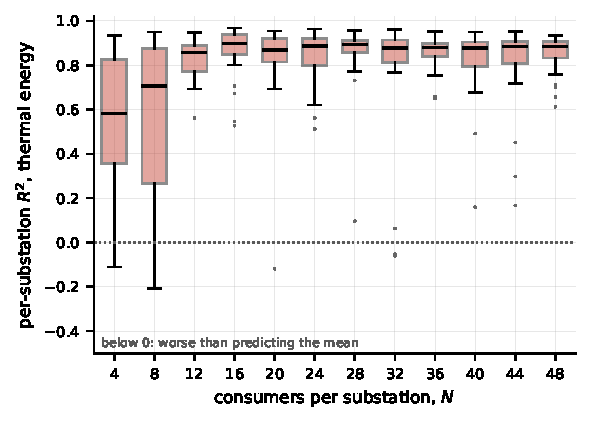
\includegraphics[width=\columnwidth]{figures/fig_energy_by_aggregation.pdf}
\caption{Per-substation accuracy of the thermal-energy estimate against consumer count, at 25\% ETL penetration. Each box holds the 25 replicates of that cell. The median rises modestly while the spread contracts sharply, so aggregation buys reliability across substations more than accuracy at the typical one. Two substations falling below the axis are not shown.}
\label{fig:energy-aggregation}
\end{figure}

The bias pooled over penetration behaves differently. It stays between $-9.9\%$ and $-12.2\%$ across the whole range of $N$, with no trend. Aggregation suppresses the variance of the estimate, and the small-sample bias that inflates it at low penetration, yet leaves the systematic shortfall untouched. That shortfall is a property of the functional form rather than of the sample, as the dead band examined below implies.

Accuracy is also not uniform across the temperature range. Splitting substation-days at the median daily mean temperature, the estimator reaches $R^2 = 0.971$ and a bias of $-2.4\%$ on cold days, against $R^2 = 0.453$ and a bias of $-54.7\%$ on warm days; RMSE is comparatively stable, at 82 and 99~kWh/day respectively. This is possibly a consequence of the dead band in Equation~\eqref{eq:thermal-response}. Above $T_h$ the thermal term is exactly zero by construction, so any ETL energy persisting into mild weather -- domestic hot water, most plausibly -- is unexplained by the estimator. A large relative bias results even where the absolute error stays modest.


\subsection{Effect of Temporal Resolution}
\label{subsection:resolution}

The two use cases do not favour the same averaging window, and neither agrees with fit quality. Section~\ref{subsection:fitquality} showed net-load $R^2$ improving monotonically as the window widens, reaching 0.948 at 24~h for a substation of 48 consumers at 50\% penetration. Detection AUC does not follow: it peaks at 4--8~h, at 0.994, and falls to 0.990 at 24~h (Fig.~\ref{fig:auc-resolution}). Resampling the same substations at every resolution, so that the comparison stays paired, confirms the difference is systematic: AUC at 4~h, 8~h and 16~h is significantly above the 24~h value, while no resolution differs significantly from 24~h in sensitivity.

The two objectives consequently point in opposite directions, though not with comparable force. Coarsening from 1~h to 24~h gains 0.22 in $R^2$ and costs at most 0.005 in AUC, with no significant sensitivity penalty. The daily aggregation adopted in Section~\ref{section:identify} is therefore warranted, provided the AUC optimum near 4--8~h is acknowledged where detection alone is the objective. Total-energy accuracy is comparatively insensitive to the fitting resolution, with $R^2$ between 0.948 and 0.953 and bias between $-11\%$ and $-13\%$ across the five resolutions tested.

\begin{figure}[t]
\centering
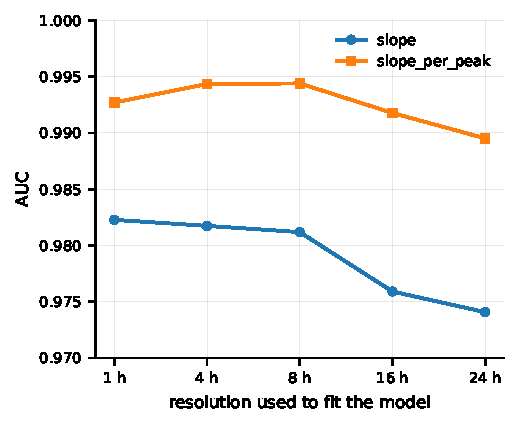
\includegraphics[width=\columnwidth]{figures/fig_s3_auc_by_resolution.pdf}
\caption{Detection AUC against the resolution used to fit the model, for the raw and the peak-normalised sensitivity.}
\label{fig:auc-resolution}
\end{figure}


\section{Discussion}
\label{section:discussion}


\subsection{Accuracy}
\label{subsection:accuracy}

Accuracy improves with aggregation, though not without limit and not in every quantity. Fit quality and Energy Estimation both rise with the consumer count, and in both cases the gain is largest where ETL penetration is lowest (Sections~\ref{subsection:fitquality} and~\ref{subsection:energy}). Aggregation is therefore most useful exactly where the ETL signal is weakest, which is the regime a DSO is likely to meet first as uptake begins. Section~\ref{subsection:reproduction} reproduces the fit-quality half of that statement on an independent dataset.

Two quantities do not follow. Detection is already at ceiling within a known consumer count, at a median AUC of 1.000 at every size tested, so aggregation has no headroom to improve it. The total-energy bias is likewise invariant, holding between $-9.9\%$ and $-12.2\%$ across the whole range of $N$. Aggregation consequently improves the precision of what the fit recovers, rather than its correctness, and the distinction matters because the two failure modes have different remedies.

The clearest weakness is the accuracy of Energy Estimation away from the coldest conditions, where $R^2$ falls from 0.971 on cold days to 0.453 on warm ones (Section~\ref{subsection:energy}). This is consistent with the dead band identified in Section~\ref{section:identify}: any ETL energy that persists above $T_h$ is unexplained by construction, not by a fitting failure, so no amount of additional data corrects it. Heat pumps commonly serve domestic hot water alongside space heating, a duty maintained throughout the year and largely independent of ambient temperature, so this share of ETL demand persists above $T_h$ regardless of season and is missed by the estimator. This marks a genuine boundary of Equation~\eqref{eq:thermal-response}, rather than a shortcoming specific to Energy Estimation. Detection is left untouched by it, since that use case reads the slope below $T_h$ and never integrates energy above it. The same fit can consequently transfer cleanly as a detector while still under-reporting annual ETL energy.


\subsection{Generalisability}
\label{subsection:generalisability}

Three datasets still provide a narrow basis for a general claim, though what Section~\ref{subsection:reproduction} establishes is broader than a single reproduction. The aggregation behaviour transfers: fit quality rises with the consumer count in WPUQ and in Austin as it does in Switzerland, over nested sequences in which each aggregate contains the one below it. It also survives a change of thermostatic technology, the Austin fit being driven by cooling rather than heating. The levels differ, at 0.845 against 0.948 for the largest aggregate at 24~h, and the direction does not. That the effect survives a change of country, climate, building stock and metering arrangement suggests it follows from aggregation itself rather than from anything particular to the training data.

The two use cases are not shown to transfer, and this should not be read as evidence that they do not. WPUQ contains no consumer without a heat pump, so a reference group of genuinely ETL-free consumers cannot be built and Detection cannot be scored without making the problem easier than it is (Section~\ref{subsection:designs}). Energy Estimation could in principle be evaluated there, yet on 37 houses from a single feeder it would rest on too narrow a base to distinguish a property of the method from a property of that feeder. Both therefore stand on the training dataset alone, and a second dataset with a genuine ETL-free population would be needed to establish either.

Absolute quantities are not expected to transfer in any case. Thermal Sensitivities reflect the local building stock, climate and heating practice, so recalibration at every new deployment is expected rather than a sign of failure. This is precisely why Section~\ref{section:identify} normalises by peak or base load rather than reporting the sensitivity directly. It is also why Section~\ref{subsection:two-effects} frames its argument in terms of what aggregation does to the fit, rather than in terms of any particular fitted value.

The temporal axis carries the same caveat as the consumer one. Coarsening the averaging window improves fit quality in both datasets, so that much generalises. Whether the detection optimum near 4--8~h reported in Section~\ref{subsection:resolution} generalises is untested, for the same reason Detection itself is untested here.

The remaining methodological choice that a third dataset would need to reproduce is how the ETL-free class is defined. Section~\ref{subsection:data} defines it negatively, as the absence of a submetered heat pump and of five surveyed heating types, so the negative class is defined rather than filtered. A dataset whose reference group is assembled by any other rule would not be measuring the same quantity, and Section~\ref{subsection:designs} shows how easily that distinction is lost where every consumer carries the load under test.

\subsection{Data Requirements}

Both use cases share the same minimal input, net load at the substation and ambient temperature. A distinction between apparatus and input is needed before going further. The household survey of Section~\ref{subsection:data} is used to build the design and to label the ground truth against which the use cases are scored, so it is required to \emph{validate} the method, not to \emph{run} it. What each use case additionally demands in operation follows from the absolute-versus-relative distinction drawn in Section~\ref{section:identify}.

The aggregation level is itself a data requirement, and an unusual one in that the results above put a value on it. Section~\ref{subsection:detection} shows a known consumer count would raise Detection to a median AUC of 1.000, against 0.990 for the normalised statistic without it. Knowing $N$ is therefore worth about 0.01 in AUC, and normalisation already recovers roughly three quarters of what its absence costs. Publishing consumer counts alongside aggregated substation consumption would improve Detection, without being a precondition for it.

Detection needs, in addition, a comparison point: either a local reference distribution built from substations known to carry no ETL, as in Section~\ref{subsection:data}, or an externally calibrated threshold. Whether a threshold calibrated elsewhere can stand in for a local reference group is not settled here, since WPUQ cannot supply an ETL-free population to test it against. What Detection does not need is the consumer count $N$ itself, since the statistic it operates on is already normalised by peak or base load.

Energy Estimation needs neither a reference group nor $N$ to report the total temperature-driven energy of a substation, the quantity validated against submetered ground truth in Section~\ref{subsection:energy}. $N$ becomes necessary only if the ETL-specific share is required rather than the total, since isolating it means subtracting the reference-group contribution $N \sigma_{\mathrm{base}}$ from Equation~\eqref{eq:sensitivity-decomposition}, as noted in Section~\ref{section:identify}.

The divergence follows from which part of Equation~\eqref{eq:thermal-response} each use case reads. The total form of Energy Estimation needs nothing beyond the fitted thermal term itself. Detection instead depends on knowing what an ETL-free substation looks like, a fact the fit cannot supply, which is why a comparison group or an equivalent threshold is unavoidable.


\subsection{Interpretability}
\label{subsection:interpretability}

Each parameter of Equation~\eqref{eq:thermal-response} carries a direct physical reading. $P_{\mathrm{base}}$ is the substation's temperature-independent load, $T_h$ and $T_c$ are balance-point temperatures at which heating and cooling loads switch on, and $s_h$ and $s_c$ are the resulting slopes. Fig.~\ref{fig:bathtub} shows these are not free parameters chosen only to fit the data well. The heating and cooling thresholds recovered from the Austin aggregate, $11.2^\circ$C and $19.8^\circ$C, sit within the range a building's thermostat set-points and envelope losses would place them. The dead band between them is exactly the interval over which neither system runs.

The heating sensitivity $s_h$ is harder to read directly, because Equation~\eqref{eq:sensitivity-decomposition} shows it is already a sum of two physically distinct contributions: the aggregate non-thermal response of $N$ ordinary consumers, and the thermal response of $N_{\mathrm{etl}}$ ETLs. A given value of $s_h$ is consistent with many $(N, N_{\mathrm{etl}})$ pairs, so the slope alone does not disclose which mechanism produced it, the same confound that Section~\ref{subsection:detection} shows can invert a naive ranking of substations by raw sensitivity. Normalisation restores comparability across substations, but not this decomposition: a peak-normalised sensitivity is still a mixture, only one whose mixture ratio is now comparable between substations of different size. Section~\ref{subsection:detection} bounds how much the mixture costs in practice. What it obstructs is the reading of a single substation's slope, rather than the discrimination between substations, which stays near-perfect once the consumer count is fixed.

Equation~\eqref{eq:thermal-response} is fitted, and should be read, only within the observed temperature range. That range differs between the two datasets, reaching $-9.6^\circ$C in Switzerland against $-5.4^\circ$C in WPUQ, so conditions that are still interpolation for one are already extrapolation for the other. The heating arm is linear without bound, whereas the load it describes cannot exceed what the installed ETLs can draw, so the fitted line must depart from the physical response at some temperature below the observed minimum. Nothing in the fit itself signals where, since the data that would locate it are exactly the data the fit does not have.

The same caution applies on the warm side. The fitted zero above $T_h$ should be read as \emph{not captured by this term} rather than as evidence that no ETL load remains, a distinction Section~\ref{subsection:accuracy} traces to the persistent domestic hot water demand the estimator misses.

Some physically meaningful quantities are not recoverable from Equation~\eqref{eq:thermal-response} at any temperature, installed ETL capacity among them, for the reason given in Section~\ref{section:identify}. Interpretability, in this sense, is bounded twice over: once by the observed temperature range, and once by what the functional form of Equation~\eqref{eq:thermal-response} was ever capable of representing.


\subsection{Concluding Remarks}

Aggregation is what renders these loads visible, and what renders them ambiguous. A single ETL cycles on and off, and its instantaneous demand says little about the temperature that drove it. Summed over a substation, the same loads produce a smooth response whose parameters are well determined and physically readable. Every result above rests on that transition, and the two use cases are not competing tools but two readings of the one fit it makes possible.

What aggregation buys is precision rather than correctness. Fit quality and the energy estimate both sharpen with the consumer count, most where the ETL signal is weakest, yet the systematic bias is invariant to aggregation, since it follows from the functional form rather than the sample. What aggregation costs is attributability, as the same summation that smooths the response also accumulates the non-ETL term of Equation~\eqref{eq:sensitivity-decomposition}, leaving a well-fitted curve ambiguous about its origin until a known consumer count or a normalisation resolves it. Two limits lie beyond aggregation altogether: the dead band, which leaves warm-weather ETL energy unrepresented, and the installed capacity, which net load never exposes.

No single aggregation level is therefore preferable across both use cases. Larger substations yield better-determined fits and more accurate energy estimates, whereas Detection is already saturated at the smallest size tested. Where a consumer count is available it is worth more than additional aggregation, and where it is not, the normalised statistic recovers most of what its absence costs -- the condition under which a DSO actually operates.


\section{Conclusion}
\label{section:conclusion}


% \bibliographystyle{IEEEtran}
% \bibliography{reference}

\end{document}